
\documentclass[../open-optimization/open-optimization.tex]{subfiles}


\begin{document}

\chapter{NLP Algorithms}


\section{Algorithms Introduction}

We will begin with unconstrained optimization and consider several different algorithms based on what is known about the objective function.  In particular, we will consider the cases where we use
\begin{itemize}
\item Only function evaluations (also known as \emph{derivative free optimization}),
\item Function and gradient evaluations,
\item Function, gradient, and hessian evaluations.
\end{itemize}

We will first look at these algorithms and their convergence rates in the 1-dimensional setting and then extend these results to higher dimensions.

\section{1-Dimensional Algorithms}
We suppose that we solve the problem 

\begin{align}
\min f(x)\\
x \in [a,b].
\end{align}

That is, we minimize the univariate function $f(x)$ on the interval $[l,u]$.  

For example, 

\begin{align}
\min (x^2 - 2)^2\\
 0 \leq x \leq 10.
\end{align}

Note, the optimal solution lies at $x^* = \sqrt{2}$, which is an irrational number.  Since we will consider algorithms using floating point precision, we will look to return a solution $\bar x$ such that $\|x^* - \bar x\| < \epsilon$ for some small $\epsilon > 0$, for instance, $\epsilon = 10^{-6}$.


\subsection{Golden Search Method - Derivative Free Algorithm}
\url{https://www.youtube.com/watch?v=hLm8xfwWYPw}

Suppose that $f(x)$ is unimodal on the interval $[a,b]$, that is, it is a continuous function that has a single minimizer on the interval.  

Without any extra information, our best guess for the optimizer is $\bar x = \tfrac{a+ b}{2}$ with a maximum error of $\epsilon = \tfrac{b-a}{2}$.    Our goal is to reduce the size of the interval where we know $x^*$ to be, and hence improve our best guess and the maximum error of our guess.


 Now we want to choose points in the interior of the interval to help us decide where the minimizer is.  Let $x_1, x_2$ such that 

$$
a < x_2 < x_1 < b.
$$

Next, we evaluate the function at these four points.  Using this information, we would like to argue a smaller interval in which $x^*$ is contained.  In particular, since $f$ is unimodal, it must hold that 
\begin{enumerate}
\item $x^* \in [a, x_2]$ if  $f(x_1) \leq f(x_2)$, 
\item $x^* \in [x_1,b]$ if $f(x_2) < f(x_1)$,
\end{enumerate}


After comparing these function values, we can reduce the size of the interval and hence reduce the region where we think $x^*$ is.   


We will now discuss how to chose $x_1,x_2$ in a way that we can 
\begin{enumerate}
\item Reuse function evaluations,
\item Have a constant multiplicative reduction in the size of the interval.
\end{enumerate}


We consider the picture:\\
%\begin{center}
%\includegraphics[scale = 0.4]{golden-search-explain}\\
%\end{center}
%In case 1, we remove the right side:\\
%\begin{center}
%\includegraphics[scale = 0.4]{golden-search-explain1}\\
%\end{center}
%In case 2, we remove the left side:\\
%\begin{center}
%\includegraphics[scale = 0.4]{golden-search-explain2}\\
%\end{center}

To determine the best $d$, we want to decrease by a constant factor.  Hence, we decrease be a factor $\gamma$, which we will see is the golden ration (GR).  To see this, we assume that $(b-a) = 1$, and ask that $d = \gamma$.  Thus, $x_1 - a = \gamma$ and $b - x_2 = \gamma$.  If we are in case 1, then we cut off $b-x_1 = 1-\gamma$.  Now, if we iterate and do this again, we will have an initial length of $\gamma$ and we want to cut off the interval $x_2 - x_1$ with this being a proportion of $(1-\gamma)$ of the remaining length.  Hence, the second time we will cut of $(1-\gamma)\gamma$, which we set as the length between $x_1$ and $x_2$.  

Considering the geometry, we have
$$
\text{ length $a$ to $x_1$ } + \text{length $x_2$ to $b$} = \text{ total length } + \text{ length $x_2$ to $x_2$}
$$ 
hence
$$
\gamma + \gamma = 1 + (1-\gamma)\gamma.
$$
Simplifying, we have
$$
\gamma^2 + \gamma - 1 = 0.
$$
Applying the quadratic formula, we see
$$
\gamma = \frac{-1 \pm \sqrt{5}}{2}.
$$
Since we want $\gamma > 0$, we take 
$$
\gamma = \frac{-1 + \sqrt{5}}{2} \approx 0.618
$$
This is exactly the Golden Ratio (or, depending on the definition, the golden ration minus 1).



\subsubsection{Example:}

%\begin{center}
%\includegraphics[scale = 0.4]{golden-search-example1}\\
%Initial setup:\\
%\includegraphics[scale = 0.4]{golden-search-example2}\\
%Step 1:\\
%\includegraphics[scale = 0.4]{golden-search-example3}\\
%Step 2:\\
%\includegraphics[scale = 0.4]{golden-search-example4}\\
%Step 3:\\
%\includegraphics[scale = 0.4]{golden-search-example5}\\
%Step 4:\\
%\includegraphics[scale = 0.4]{golden-search-example6}
%\end{center}
We can conclude that the optimal solution is in $[1.4,3.8]$, so we would guess the midpoint $\bar x = 2.6$ as our approximate solution with a maximum error of $\epsilon = 1.2$.

\begin{general}{Convergence Analysis of Golden Search Method}{}
After $t$ steps of the Golden Search Method, the interval in question will be of length
$$
(b-a)(GR)^t \approx (b-a)(0.618)^t
$$
Hence, by guessing the midpoint, our worst error could be
$$
\frac{1}{2}(b-a)(0.618)^t.
$$
\end{general}






\subsection{Bisection Method - 1st Order Method (using Derivative)}

\subsubsection{Minimization Interpretation}
\textbf{Assumptions: $f$ is convex, differentiable}\\

We can look for a minimizer of the function $f(x)$ on the interval $[a,b]$.


\subsubsection{Root finding Interpretation}
Instead of minimizing, we can look for a root of $f'(x)$.  That is, find $x$ such that $f'(x) = 0$.  

\textbf{Assumptions: $f'(a)<0 <  f'(b)$, OR, $f'(b) < 0 < f'(a)$.  $f'$ is continuous}\\
The goal is to find a root of the function $f'(x)$ on the interval $[a,b]$.  If $f$ is convex, then we know that this root is indeed a global minimizer.


Note that if $f$ is convex, it only makes sense to have the assumption $f'(a)<0 <  f'(b)$.






\begin{general}{Convergence Analysis of Bisection Method}{}
After $t$ steps of the Bisection Method, the interval in question will be of length
$$
(b-a)\left(\frac{1}{2}\right)^t.
$$
Hence, by guessing the midpoint, our worst error could be
$$
\frac{1}{2}(b-a)\left(\frac{1}{2}\right)^t.
$$
\end{general}

\subsection{Gradient Descent - 1st Order Method (using Derivative)}
\textbf{Input:} $f(x)$, $\nabla f(x)$, initial guess $x^0$, learning rate $\alpha$, tolerance $\epsilon$\\
\textbf{Output:} An approximate solution $x$

\begin{enumerate}
\item Set $t= 0$
\item While $\| f(x^t)\|_2 > \epsilon$:
\begin{enumerate}
\item Set $x^{t+1} \leftarrow x^t- \alpha \nabla f(x^t)$.
\item Set $t \leftarrow t+1$.
\end{enumerate}
\item Return $x^{t}$.
\end{enumerate}



\subsection{Newton's Method - 2nd Order Method (using Derivative and Hessian)}

\textbf{Input:} $f(x)$, $\nabla f(x)$, $\nabla^2f(x)$, initial guess $x^0$, learning rate $\alpha$, tolerance $\epsilon$\\
\textbf{Output:} An approximate solution $x$

\begin{enumerate}
\item Set $t= 0$
\item While $\| f(x^t)\|_2 > \epsilon$:
\begin{enumerate}
\item Set $x^{t+1} \leftarrow x^t - \alpha [\nabla^2 f(x^t)]^{-1} \nabla f(x^t)$.
\item Set $t \leftarrow t+1$.
\end{enumerate}
\item Return $x^t$.
\end{enumerate}


\section{Multi-Variate Unconstrained Optimizaition}
We will now use the techniques for 1-Dimensional optimization and extend them to multi-variate case.  We will begin with unconstrained versions (or at least, constrained to a large box) and then show how we can apply these techniques to constrained optimization.

\subsection{Descent Methods - Unconstrained Optimization - Gradient, Newton} 

\begin{general}{Outline for Descent Method for Unconstrained Optimization}{}
\textbf{Input:} 
\begin{itemize}
\item A function $f(x)$
\item Initial solution $x^0$
\item Method for computing step direction $d_t$
\item Method for computing length $t$ of step
\item Number of iterations $T$
\end{itemize}

\textbf{Output:}
\begin{itemize}
\item A point $x_{T}$ (hopefully an approximate minimizer)
\end{itemize}

\textbf{Algorithm}
\begin{enumerate}
\item For $t=1, \dots, T$,
$$
\text{ set } x_{t+1} = x_t + \alpha_t d_t 
$$
\end{enumerate}

\end{general}
\subsubsection{Choice of $\alpha_t$}
There are many different ways to choose the step length $\alpha_t$.  Some choices have proofs that the algorithm will converge quickly.  An easy choice is to have a constant step length $\alpha_t = \alpha$, but this may depend on the specific problem.

\subsubsection{Choice of $d_t$ using $\nabla f(x)$}
Choice of descent methods using $\nabla f(x)$ are known as \emph{first order methods}.
Here are some choices:
\begin{enumerate}
\item \textbf{Gradient Descent:}   $d_t = - \nabla f(x_t)$
\item \textbf{Nesterov Accelerated Descent:} $d_t = \mu (x_t - x_{t-1}) - \gamma \nabla f(x_t + \mu(x_t- x_{t-1}))$
\end{enumerate}
Here, $\mu, \gamma$ are some numbers.  The number $\mu$ is called the momentum.  

\subsection{Stochastic Gradient Descent - The mother of all algorithms.}
 A popular method is called \emph{stochastic gradient descent} (SGD).   This has been described as "The mother of all algorithms".  
 This is a method to \textbf{approximate the gradient} typically used in machine learning or stochastic programming settings.  
 
\begin{general}{Stochastic Gradient Descent}{}

Suppose we want to solve
\begin{equation}
\min_{x \in \R^n} F(x) = \sum_{i=1}^N f_i(x).
\end{equation}

We could use \emph{gradient descent} and have to compute the gradient $\nabla F(x)$ at each iteration.  But!   We see that in the \textbf{cost to compute the gradient} is roughly $O(nN)$, that is, it is very dependent on the number of function $N$, and hence each iteration will take time dependent on $N$.

\textbf{Instead!} Let $i$ be a uniformly random sample from $\{1, \dots, N\}$.  Then we will use $\nabla f_i(x)$ as an approximation of $\nabla F(x)$.  Although we lose a bit by using a guess of the gradient, this approximation only takes $O(n)$ time to compute.  And in fact, in expectation, we are doing the same thing.  That is,

$$
N\cdot  \mathbb{E}( \nabla f_i(x)) = N \sum_{i=1}^N \frac{1}{N} \nabla f_i(x) =  \sum_{i=1}^N\nabla f_i(x) = \nabla \left(  \sum_{i=1}^N   f_i(x)\right) = \nabla F(x).
$$


Hence, the SGD algorithm is:

\begin{enumerate}
\item Set $t = 0$
\item While ...(some stopping criterion)
\begin{enumerate}
\item Choose $i$ uniformly at random in $\{1, \dots, N\}$.
\item Set $d_t = \nabla f_i(x_t)$
\item Set $x_{t+1} = x_t - \alpha d_t$
\end{enumerate}
\end{enumerate}

There can be many variations on how to decide which functions $f_i$ to evaluate gradient information on.  Above is just one example.

\end{general}
 
 
 
 Linear regression is an excellent example of this.  

\begin{example}{Linear Regression with SGD}{}
Given data points $x^1, \dots, x^N \in \R^d$ and output $y^1, \dots, y^N \in \R$, find $a \in \R^d$ and $b \in \R$ such that $a^\top x^i + b \approx y^i$.   This can be written as the optimization problem 
\begin{equation}
\begin{array}{rl}
\min_{a,b} \quad & \sum_{i=1}^N g_i(a,b)
\end{array}
\end{equation}
where $g_i(a,b) = (a^\top x^i + b)^2$.   

Notice that the objective function $G(a,b) = \sum_{i=1}^N g_i(a,b)$  is a convex quadratic function.  The gradient of the objective function is 
$$
\nabla G(a,b) = \sum_{i=1}^N \nabla g_i(a,b) = \sum_{i=1}^N 2x^i (a^\top x^i + b)
$$

Hence, if we want to use gradient descent, we must compute this large sum (think of $N \approx 10,000$).  

Instead, we can \textbf{approximate the gradient!}.  Let $\tilde \nabla G(a,b)$ be our approximate gradient.  We will compute this by randomly choosing a value $r \in \{1, \dots, N\}$ (with uniform probability).  Then set

$$
\tilde \nabla G(a,b) = \nabla g_r(a,b).
$$

It holds that the expected value is the same as the gradient, that is,

$$
\mathbb{E}(\tilde \nabla G(a,b)) = G(a,b).
$$


Hence, we can make probabilistic arguments that these two will have the same (or similar) convergence properties (in expectation).
\end{example}



\subsubsection{Choice of $\Delta_k$ using the hessian $\nabla^2 f(x)$}
These choices are called \emph{second order methods}
\begin{enumerate}
\item \textbf{Newton's Method:}   $\Delta_k = - (\nabla^2f(x_k))^{-1} \nabla f(x_k)$
\item \textbf{BFGS (Quasi-Newton):} $\Delta_k = - (B_k)^{-1} \nabla f(x_k)$
\end{enumerate}
Here
\begin{align*}
s_k &= x_{k+1} - x_k\\
y_k &= \nabla f(x_{k+1}) - \nabla f(x_k)
\end{align*}
and
$$
B_{k+1} = B_k - \frac{(B_k s_k)(B_k s_k)^\top}{s_k^\top B_k s_k} + \frac{y_k y_k^\top}{y_k^\top s_k}.
$$
This serves as an approximation of the hessian and can be efficiently computed.  Furthermore,  the inverse can be easily computed using certain updating rules.  This makes for a fast way to approximate the hessian.



\section{Constrained Convex Nonlinear Programming}
Given a convex function $f(x)\colon \R^d \to \R$ and convex functions $f_i(x)\colon \R^d \to \R$ for $i=1, \dots, m$,  the \emph{convex programming} problem is
\begin{equation}
\label{eq:convex-programming-for-example}
\begin{split}
\min \quad & f(x)\\
\st  \quad & f_i(x) \leq 0  \quad  \text{ for } i=1, \dots, m\\
& x \in \R^d
\end{split}
\end{equation}

\subsection{Barrier Method}
\begin{general}{Constrained Convex Programming via Barrier Method}{}
We convert~\eqref{eq:convex-programming-for-example} into the unconstrained minimization problem:
\begin{equation}
\label{eq:convex-programming-barrier}
\begin{split}
\min \quad & f(x) - \phi \sum_{i=1}^m \log(-f_i(x)) \\
& x \in \R^d
\end{split}
\end{equation}
Here $\phi > 0$ is some number that we choose.  As $\phi \to 0$, the optimal solution $x(\phi)$ to \eqref{eq:convex-programming-barrier} tends to the optimal solution of \eqref{eq:convex-programming-for-example}.  That is $x(\phi) \to x^*$ as $\phi \to 0$.
\end{general}

\begin{general}{Constrained Convex Programming via Barrier Method - Initial solution}{}
Define a variable $s \in \R$ and add that to the right hand side of the inequalities and then minimize it in the objective function.
\begin{equation}
\label{eq:convex-programming}
\begin{split}
\min \quad & s\\
\st  \quad & f_i(x) \leq s \quad  \text{ for } i=1, \dots, m\\
& x \in \R^d, s \in \R
\end{split}
\end{equation}
Note that this problem is feasible for all $x$ values since $s$ can always be made larger.  
If there exists a solution with $s \leq 0$, then we can use the corresponding $x$ solution as an initial feasible solution.  Otherwise, the problem is infeasible.

Now, convert this problem into the unconstrained minimization problem:
\begin{equation}
\label{eq:convex-programming}
\begin{split}
\min \quad & f(x) - \phi \sum_{i=1}^m \log(-(f_i(x)-s)) \\
& x \in \R^d, s \in \R
\end{split}
\end{equation}
This problem has an easy time of finding an initial feasible solution.  For instance, let $x = 0$, and then $s = \max_i f_i(x) +1 $.  
\end{general}


\textbf{Images below: the value $t$ is the value $\phi$ discussed above}
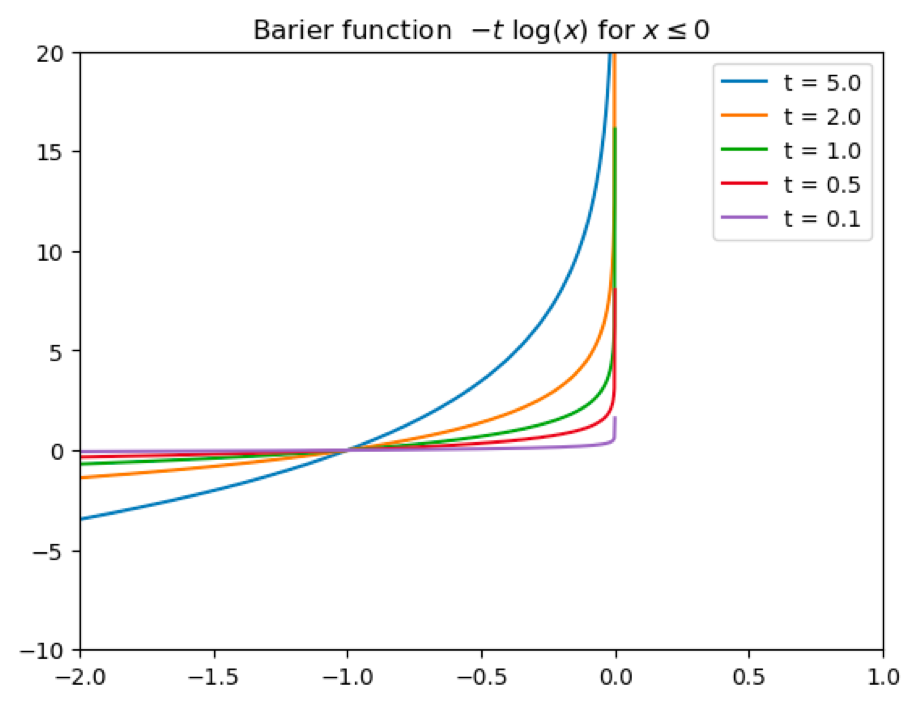
\includegraphics[scale = 0.4]{barrier-function}
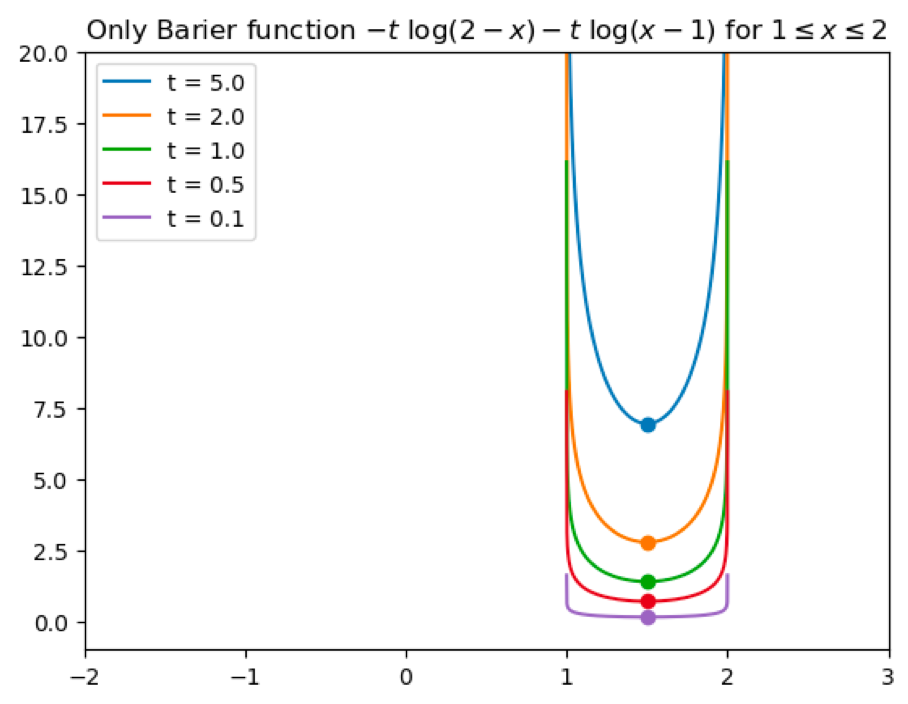
\includegraphics[scale = 0.4]{barrier-functions-added}
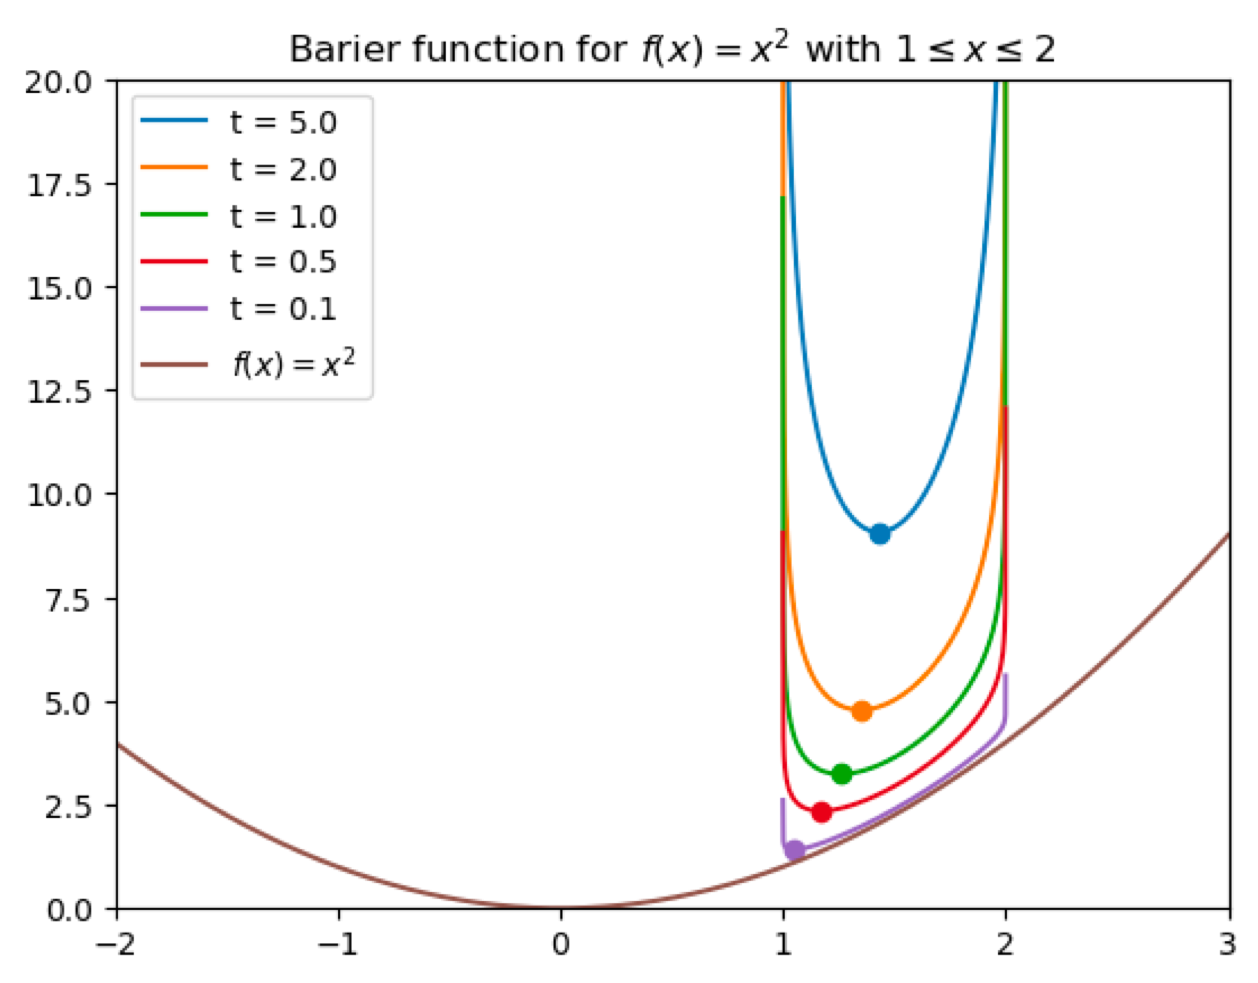
\includegraphics[scale = 0.4]{barrier-method}
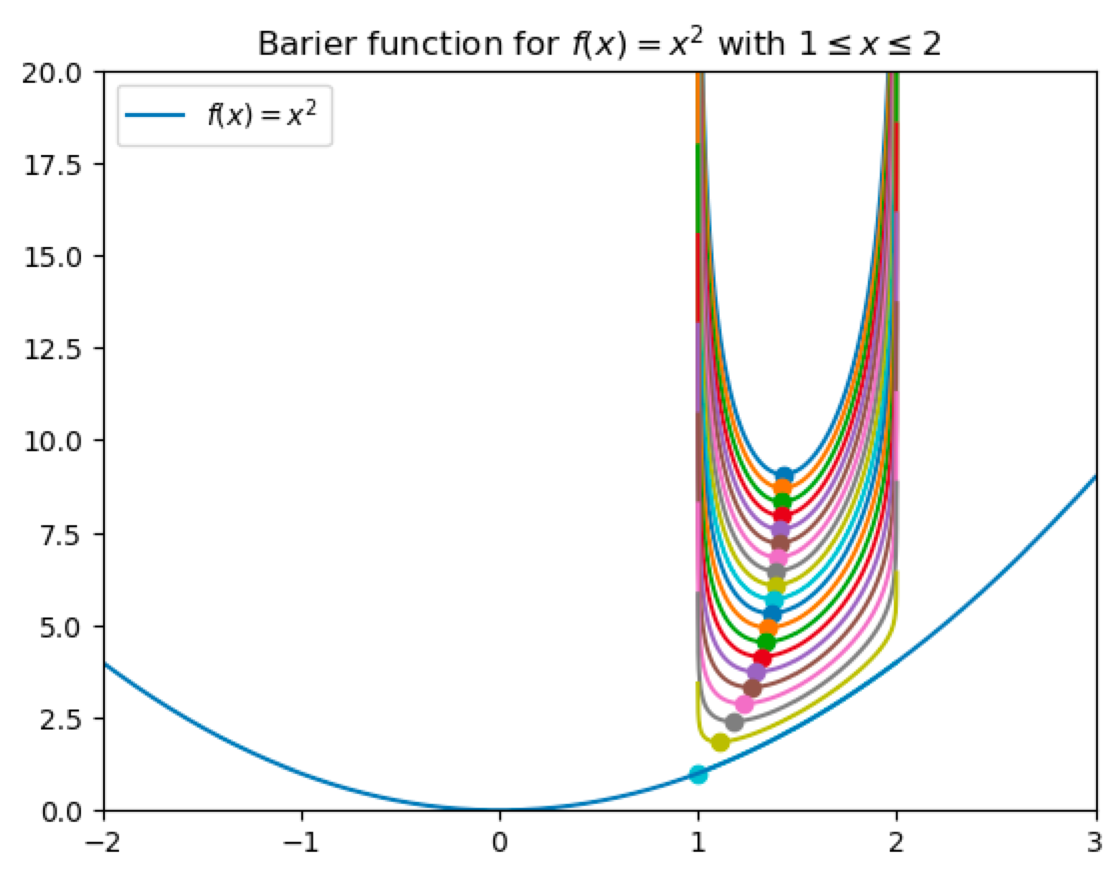
\includegraphics[scale = 0.4]{central-path1}
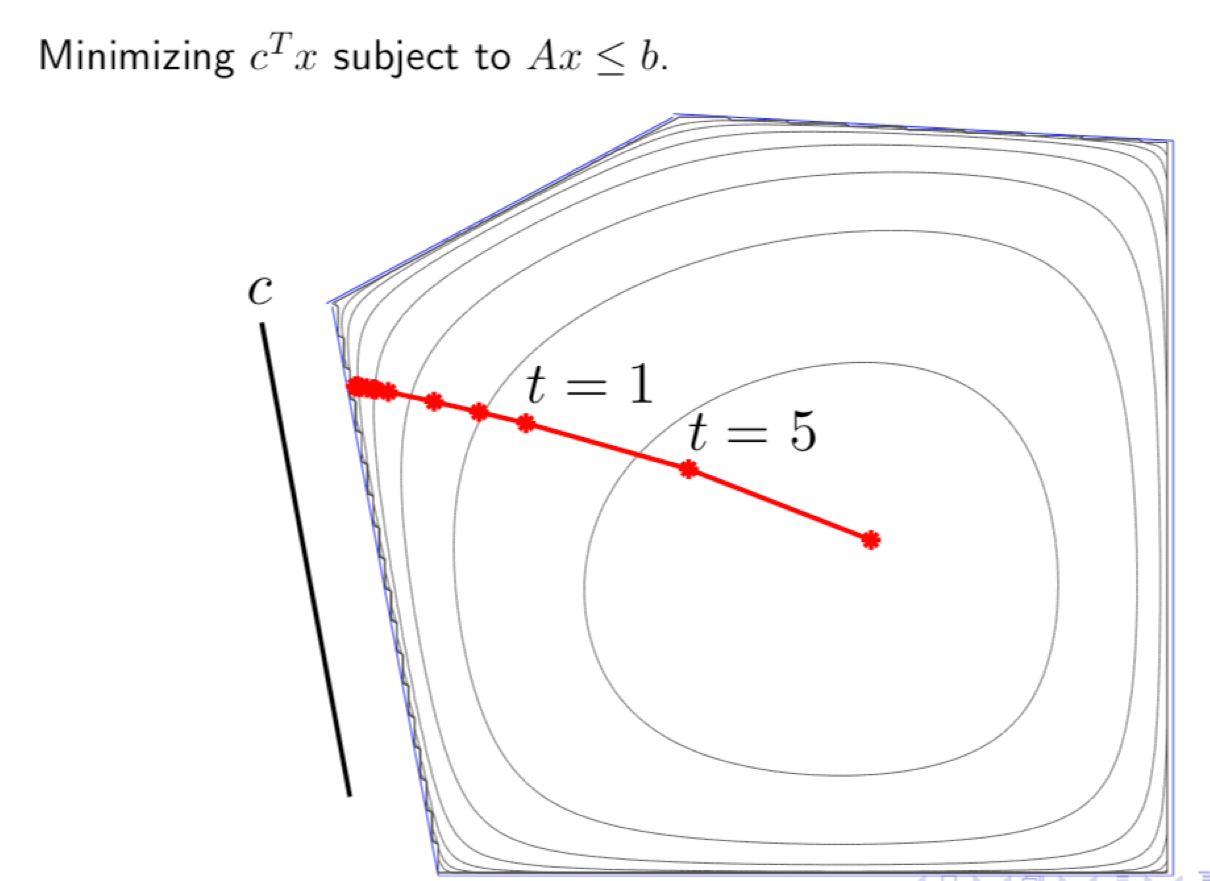
\includegraphics[scale = 0.4]{central-path2}\footnote{Image taken from unknown source.}


\chapter{Computational Issues with NLP}
We mention a few computational issues to consider with nonlinear programs.  
\section{Irrational Solutions}
Consider nonlinear problem (this  is even convex)
\begin{equation}
\begin{array}{rl}
\min \quad & -x\\
\text{s.t.} \quad & x^2 \leq 2.
\end{array}
\end{equation}
The optimal solution is $x^* = \sqrt{2}$, which cannot be easily represented.  Hence, we would settle for an \textbf{approximate solution} such as $\bar x = 1.41421$, which is feasible since $\bar x^2 \leq 2$, and it is close to optimal.

\section{Discrete Solutions}
Consider nonlinear problem (not convex)
\begin{equation}
\begin{array}{rl}
\min \quad & -x\\
\text{s.t.} \quad & x^2 = 2.
\end{array}
\end{equation}
Just as before, the optimal solution is $x^* = \sqrt{2}$, which cannot be easily represented.  Furthermore, the only two feasible solutions are $\sqrt{2}$ and $-\sqrt{2}$.  Thus, there is no chance to write down a feasible rational approximation.

\section{Convex NLP Harder than LP}
Convex NLP is typically polynomially solvable.  It is a generalization of linear programming.  
\begin{general}{Convex Programming}{\polynomial\ \  (typically)}
Given a convex function $f(x)\colon \R^d \to \R$ and convex functions $f_i(x)\colon \R^d \to \R$ for $i=1, \dots, m$,  the \emph{convex programming} problem is
\begin{equation}
\label{eq:convex-programming}
\begin{split}
\min \quad & f(x)\\
\st  \quad & f_i(x) \leq 0  \quad  \text{ for } i=1, \dots, m\\
& x \in \R^d
\end{split}
\end{equation}
\end{general}
\begin{example}
Convex programming is a generalization of linear programming.  This can be seen by letting $f(x) = c^\top x$ and $f_i(x) = A_i x - b_i$.  
\end{example}


\section{NLP is harder than IP}
As seen above, quadratic constraints can be used to create a feasible region with discrete solutions.  For example 
$$
x(1-x) = 0
$$
has exactly two solutions: $x = 0, x=1$.  
Thus, quadratic constraints can be used to model binary constraints.
\begin{general}{Binary Integer programming (BIP) as a NLP}{\nphard}
Given a matrix $A \in \R^{m\times n}$, vector $b \in \R^m$ and vector $c \in \R^n$, the \emph{binary integer programming} problem is
\begin{equation}
\label{eq:BIP}
\begin{split}
\max \quad & c^\top x\\
\st  \quad & Ax \leq b\\
& \hcancel[1.5pt]{x \in \{0,1\}^n}\\
& x_i(1-x_i) = 0 \quad \text{ for } i=1, \dots, n
\end{split}
\end{equation}
\end{general}


 
\section{Karush-Huhn-Tucker (KKT) Conditions}

The KKT conditions use the augmented Lagrangian problem to describe sufficient conditions for optimality of a convex program.  


\begin{general}{KKT Conditions for Optimality}{}
Given a convex function $f(x)\colon \R^d \to \R$ and convex functions $g_i(x)\colon \R^d \to \R$ for $i=1, \dots, m$,  the \emph{convex programming} problem is
\begin{equation}
\label{eq:convex-programming-KKT}
\begin{split}
\min \quad & f(x)\\
\st  \quad & g_i(x) \leq 0  \quad  \text{ for } i=1, \dots, m\\
& x \in \R^d
\end{split}
\end{equation}

Given $(\bar x, \bar \lambda)$ with $\bar x \in \R^d$ and $\bar \lambda \in \R^m$, if the KKT conditions hold, then $\bar x$ is optimal for the convex programming problem.  

The KKT conditions are
\begin{enumerate}
\item (Stationary).   
\begin{equation}
- \nabla f(\bar x) = \sum_{i=1}^m \bar \lambda_i \nabla g_i(\bar x)\\
\end{equation}
\item (Complimentary Slackness).   
\begin{equation}
 \bar \lambda_i  g_i(\bar x) = 0 \text{ for } i=1, \dots, m\\
\end{equation}
\item (Primal Feasibility).   
\begin{equation}
  g_i(\bar x) \leq 0 \text{ for } i=1, \dots, m\\
\end{equation}
\item (Dual Feasibility).   
\begin{equation}
 \bar \lambda_i \geq 0 \text{ for } i=1, \dots, m\\
\end{equation}
\end{enumerate}
\end{general}

If certain properties are true of the convex program, then every optimizer has these properties.   In particular, this holds for Linear Programming.


\section{Gradient Free Algorithms}


\subsection{Needler-Mead}

\url{https://en.wikipedia.org/wiki/Nelder%E2%80%93Mead_method}
\url{https://youtube/NI3WllrvWoc?t=96}





\chapter{Material to add...}

\subsection{Bisection Method and Newton's Method}
See section 4 of the following nodes:
\url{http://www.seas.ucla.edu/~vandenbe/133A/133A-notes.pdf}

\section{Gradient Descent}
Recap Gradient and Directional Derivatives:
\url{https://www.youtube.com/watch?v=tIpKfDc295M}

\url{https://www.youtube.com/watch?v=_-02ze7tf08}

\url{https://www.youtube.com/watch?v=N_ZRcLheNv0}

\url{https://www.youtube.com/watch?v=4RBkIJPG6Yo}




Idea of Gradient descent:
\url{https://youtu.be/IHZwWFHWa-w?t=323}

Vectors:
\url{https://www.youtube.com/watch?v=fNk_zzaMoSs&list=PLZHQObOWTQDPD3MizzM2xVFitgF8hE_ab&index=2&t=0s}





\section{Projection Gradient Methods}
\begin{figure}{h}
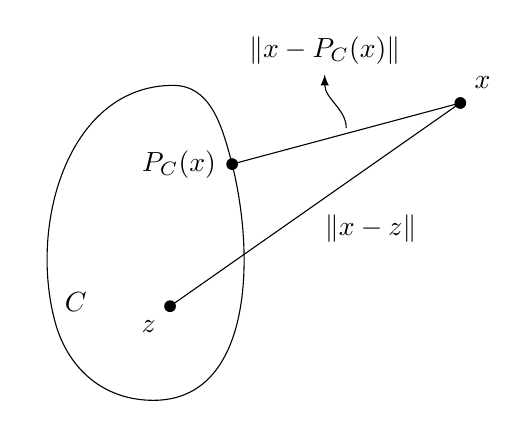
\begin{tikzpicture}[bullet/.style={circle,fill,inner sep=1.5pt,node contents={}}]
 \draw (0,0) node[bullet,label=left:$P_C(x)$,alias=PC]  -- (15:3) coordinate[midway] (aux)
    node[bullet,label=above right:$x$] -- ++ (-145:4.5) node[midway,below right]{$\|x-z\|$}     node[bullet,label=below left:$z$];
 \draw (PC) to[out=105,in=0] ++ (-0.75,1) to[out=180,in=105] ++ (-1.5,-3)
 node[above right]{$C$} to[out=-75,in=180] ++ (1.25,-1) to[out=0,in=-75] cycle;
 \draw[shorten <=2pt,-latex] (aux) to[out=90,in=-90] ++ (110:0.8) node[above]{$\|x-P_C(x)\|$};
\end{tikzpicture}
%https://tex.stackexchange.com/questions/497589/drawing-a-projection-on-closed-convex-with-tikz

\end{figure}




\end{document}
